%%%%%%%%%%%%%%%%%%%%%%%%%%%%%%%%%%%%%%%%%%%% 

\newcommand{\AgHeader}[1]{\multicolumn{3}{c}{\begin{small}
      #1 \end{small} } \\ \hline}
\newcommand{\AgNonTerm}[2] {\textsc{#1}$_{#2}$}
\newcommand{\AgAdNonTerm}[2] {\underline{\textsc{#1}}$_{#2}$}
\newcommand{\AgRule}[2] { #1 $\mapsto$ #2 }
\newcommand{\AgEmpty}[1] { & & #1 }
\newcommand{\AgRange}[2] {$#1 = 1, \dots, #2$}


% This paper: apply hybrid stochastic variational inference to adaptor grammars
% Outline
% - Brief review of adaptor grammars
% - Brief review of hybrid stochastic variational inference
% - How we put the two together
% - How well it works

\begin{frame}{Adaptor Grammars}

  \begin{columns}
    \column{.3\linewidth}
       \begin{block}{PCFG}
         \only<1>{\gfx{pcfg_00}{.9}}

       \end{block}
    \column{.65\linewidth}
        \begin{block}{Adaptor Grammars}
         \only<7>{\gfx{ag_00}{.9}}
         \only<19>{\gfx{ag_11}{.9}}
      \end{block}
      \end{columns}
\end{frame}

% Adaptor grammars
% PY Process on top of PCFGS
% Handy intuition: it caches subtrees
% compare / contrast two generative processes

% How does it do this
% CRP metaphor

% Now you can hopefully see why inference is hard
% Unbounded set of combinatorial objects
% Sampling is slow and hard (but folks try to make it better)
% Can we use online inference?

% Online variational inference
% set of parameters
% take stochastic gradient step
% what's the catch: parameters correspond to derviations (unbounded)

\begin{frame}{Why Adaptor Grammars?}
  \begin{center}
      Adaptor grammars $\equiv$ flexible ways of expressing
      probabilistic models
    \vspace{2mm}

    \pause

    \resizebox{.95\linewidth}{!}{
      \begin{tabular}{c | c | c | c}
        \textsc{PCFG}
        & 
        \begin{tabular}{l}
          Word $\mapsto$ Stem Suffix\\
          Word $\mapsto$ Stem\\
          \underline{Stem} $\mapsto$ Chars\\
          \underline{Suffix} $\mapsto$ Chars\\
          Chars $\mapsto$ Char Chars\\
          Chars $\mapsto$ Char\\
          Char $\mapsto$ ``a''\\
          $\ldots$\\
          Char $\mapsto$ ``z''\\
        \end{tabular}
        &
        \begin{tabular}{l}
          Sent $\mapsto$ Doc$^\prime_j$\\
          Doc$^\prime_j$ $\mapsto$ $\#j$\\
          Doc$^\prime_j$ $\mapsto$ Doc$^\prime_j$ Doc$_j$\\
          Doc$_j$ $\mapsto$ Topic$_i$\\
          \underline{Topic}$_i$ $\mapsto$ Word\\
          Word $\mapsto$ ``hello''\\
          \ldots\\
          Word $\mapsto$ ``world''\\
        \end{tabular}
        &
        \begin{tabular}{l}
          Sent $\mapsto$ Words\\
          Words $\mapsto$ Word Words\\
          Words $\mapsto$ Word\\
          \underline{Word} $\mapsto$ Chars\\
          Chars $\mapsto$ Char Chars\\
          Chars $\mapsto$ Char\\
          Char $\mapsto$ $a$\\
          \ldots\\
          Char $\mapsto$ $z$\\
        \end{tabular}
        \\
        \hline
        \multirow{3}{*}{input}
        &
        \multirow{3}{*}{$w$ $a$ $l$ $k$ $e$ $d$}
        &
        $\#2$ ``twitter'' ``shares''
        &
        \multirow{3}{*}{$h$ $o$ $w$ $a$ $r$ $e$ $y$ $o$ $u$}
        \\
        &
        &
        ``ipo'' ``make'' ``smooth''
        &
        \\
        &
        &
        ``market'' ``debut'' \ldots
        &
        \\
        \hline
        output
        &
        % \onslide<2->{
        \begin{tabular}{l}
          \Tree [.Word \qroof{$w$ $a$ $l$ $k$}.Stem \qroof{$e$
            $d$}.Suffix ]
        \end{tabular}
        % }
        &
        % \onslide<3->{
        \begin{tabular}{l}
          \Tree [.Doc$_2$ $\#2$ [ [ ``twitter'' ].Topic$_3$ $\ldots$
          ].Doc$_2$ ]
        \end{tabular}
        % }
        &
        % \onslide<4->{
        \begin{tabular}{l}
          \Tree [.Words \qroof{ $h$ $o$ $w$ }.Word [.Words
          \qroof{ $a$ $r$ $e$ }.Word [.Words $\ldots$ ] ] ]
        \end{tabular}
        % } 
        \\
        \hline
        model
        &
        % \onslide<2->{
        Stemmer
        % }
        &
        % \onslide<3->{
        Topic Models
        % }
        &
        % \onslide<4->{
        Word Segmention
        % }
        \\
      \end{tabular}
    }
  \end{center}
\end{frame}

\begin{frame}{Adaptor Grammars for Large Data?}
  \vspace{-1mm}
  \begin{block}{Adaptor grammar is slow!}
    \begin{itemize}
    \item MCMC inference for adaptor grammars~\citep{johnson-06}
      \begin{itemize}
      \item Pro: flexible number of adapted rules
      \item Con: non-trivial to parallelize, a lot of bookkeeping on
        the counts
      \end{itemize}
    \item Batch mode variational inference~\citep{cohen-10}
      \begin{itemize}
      \item Pro: intuitive and easy to parallelize
      \item Con: fixed number of adapted rules, require pre-processing step
      \end{itemize}
    \end{itemize}
  \end{block}

  % \begin{block}{Scale up adaptor grammar}
  %   \begin{itemize}
  %   \item Adaptor grammar with online hybrid inference
  %   \item Hybrid \textsc{MCMC}-variational: stochastic sample parameters
  %   \item Online variational inference: one pass over the dataset
  %   \item Truncation-free update: incorporate new adapted rules
  %   \end{itemize}
  % \end{block}

  \onslide<2->{
    \vspace{-1mm}
    \begin{columns}
      \column{.55\linewidth}
      \begin{center}
        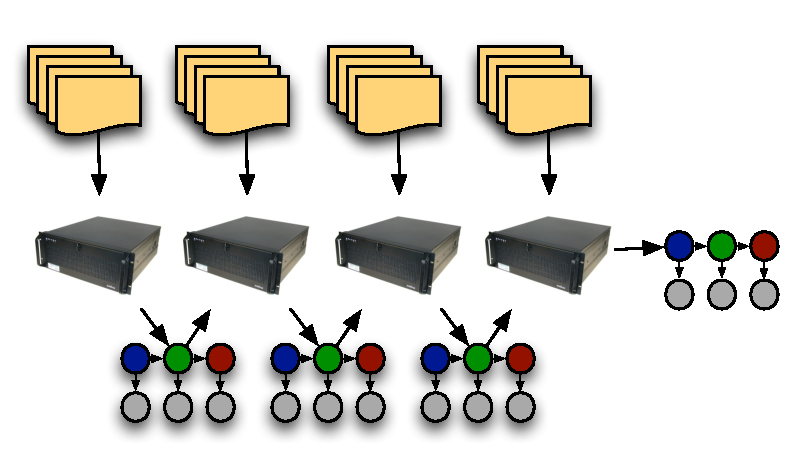
\includegraphics[width=\linewidth]{onlineag/streaming}
      \end{center}
      
      \column{.4\linewidth}
      \vspace{1mm}
      \begin{tabular}{c}
        \Tree [.Words \qroof{ $h$ $o$ $w$ }.Word [.Words
        \qroof{ $a$ $r$ $e$ }.Word [.Words $\ldots$ ] ] ]
      \end{tabular}
    \end{columns}

    \begin{center}
      Online Adaptor Grammars
    \end{center}
  }
\end{frame}

\begin{frame}{Online Adaptor Grammars}
  \begin{columns}
    \hspace{-10mm}
    \column{0.4\linewidth}
    \resizebox{1.15\linewidth}{!}{
      \begin{tabular}{c l c}
        & \multicolumn{2}{r}{\textsc{Word}} \\
        & Word $\mapsto$ Stem Suffix & 0.7\\
        & Word $\mapsto$ Stem & 0.3\\
        & \multicolumn{2}{r}{\underline{\textsc{Stem}}} \\
        \only<1,2>{
          & Stem $\mapsto$ Chars & 1
        }
        \only<3,4>{
          & Stem $\mapsto$ Chars & \alert<3>{0.91}
        }
        \only<5,6>{
          & Stem $\mapsto$ Chars & \alert<5>{0.835}
        }
        \only<7>{
          & Stem $\mapsto$ Chars & \alert<7>{0.821}
        }
        \only<8,9>{
          & Stem $\mapsto$ Chars & \alert<8>{0.32}
        }
        \only<1->{\\}
        \only<3,4>{
          & \alert<3>{Stem $\mapsto$ ``a'' ``s'' ``k''} & \alert<3>{0.09}
        }
        \only<5,6>{
          & Stem $\mapsto$ ``a'' ``s'' ``k'' & \alert<5>{0.083}
        }
        \only<7>{
          & Stem $\mapsto$ ``a'' ``s'' ``k'' & \alert{0.084}
        }
        \only<8,9>{
          & Stem $\mapsto$ ``a'' ``s'' ``k'' & \alert<8>{0.079}
        }
        \only<3->{\\}
        \only<5,6>{
          & \alert<5>{Stem $\mapsto$ ``j'' ``u'' ``m'' ``p''} &
          \alert<5>{0.082}
        }
        \only<7>{
          & Stem $\mapsto$ ``j'' ``u'' ``m'' ``p'' & \alert{0.095}
        }
        \only<8,9>{
          & Stem $\mapsto$ ``j'' ``u'' ``m'' ``p'' & \alert<8>{0.078}
        }       
        \only<5->{\\}
        \only<8,9>{
          & \alert<8>{\ldots} & \alert<8>{\ldots}
        }
        \only<8->{\\}
        & \multicolumn{2}{r}{\underline{\textsc{Suffix}}} \\
        \only<1,2>{ 
          & Suffix $\mapsto$ Chars & 1}
        \only<3,4>{     
          & Suffix $\mapsto$ Chars & \alert<3>{0.89}
        }
        \only<5,6>{     
          & Suffix $\mapsto$ Chars & \alert<5>{0.85}
        }
        \only<7>{
          & Suffix $\mapsto$ Chars & \alert<7>{0.81}
        }
        \only<8,9>{
          & Suffix $\mapsto$ Chars & \alert<8>{0.28}
        }
        \only<1->{\\}
        \only<3>{
          & \alert{Suffix $\mapsto$ ``i'' ``n'' ``g''} & \alert{0.11}
        }
        \only<4>{
          & Suffix $\mapsto$ ``i'' ``n'' ``g'' & 0.11
        }
        \only<5>{
          & Suffix $\mapsto$ ``i'' ``n'' ``g'' & \alert{0.15}
        }
        \only<6>{
          & Suffix $\mapsto$ ``i'' ``n'' ``g'' & 0.15
        }
        \only<7>{
          & Suffix $\mapsto$ ``i'' ``n'' ``g'' & \alert{0.1}
        }
        \only<8,9>{
          & Suffix $\mapsto$ ``i'' ``n'' ``g'' & \alert<8>{0.09}
        }
        \only<3->{\\}
        \only<7>{
          & \alert{Suffix $\mapsto$ ``e'' ``d''} & \alert{0.09}
        }
        \only<8,9>{
          & Suffix $\mapsto$ ``e'' ``d'' & \alert<8>{0.084}
        }
        \only<7->{\\}
        \only<8>{
          & \alert{\ldots} & \alert{\ldots}
        }
        \only<9->{
          & \ldots & \ldots
        }
        \only<8->{\\}
        & \multicolumn{2}{r}{\textsc{Chars}} \\
        & Chars $\mapsto$ Char Chars & 0.6\\
        & Chars $\mapsto$ Char & 0.4\\
        & \multicolumn{2}{r}{\textsc{Char}} \\
        & Char $\mapsto$ ``a'' & 0.11\\
        & $\ldots$ & $\ldots$\\
        & Char $\mapsto$ ``z'' & 0.009
      \end{tabular}
    }

    \only<8->{
      \column{0.05\linewidth}
    }

    \column{0.55\linewidth}
    \vspace{-6mm}
    \begin{center}
      \only<2,3>{
        \begin{scriptsize}
          \Tree [
          [
          [
          [ $a$ ].Char
          [ 
          [ $s$ ].Char
          [ 
          [ $k$ ].Char
          ].Chars
          ].Chars
          ].Chars
          ].Stem
          [
          [
          [ $i$ ].Char
          [ 
          [ $n$ ].Char
          [ 
          [ $g$ ].Char
          ].Chars
          ].Chars
          ].Chars
          ].Suffix
          ].Word
        \end{scriptsize}
      }
      \only<4,5>{
        \begin{scriptsize}
          \Tree [
          [
          [
          [ $j$ ].Char
          [ 
          [ $u$ ].Char
          [ 
          [ $m$ ].Char
          [ 
          [ $p$ ].Char
          ].Chars
          ].Chars
          ].Chars
          ].Chars
          ].Stem
          [
          [
          [ $i$ ].Char
          [ 
          [ $n$ ].Char
          [ 
          [ $g$ ].Char
          ].Chars
          ].Chars
          ].Chars
          ].Suffix
          ].Word
        \end{scriptsize}
      }
      \only<6,7>{
        \begin{scriptsize}
          \Tree [
          [
          [
          [ $j$ ].Char
          [ 
          [ $u$ ].Char
          [ 
          [ $m$ ].Char
          [ 
          [ $p$ ].Char
          ].Chars
          ].Chars
          ].Chars
          ].Chars
          ].Stem
          [
          [
          [ $e$ ].Char
          [ 
          [ $d$ ].Char
          ].Chars
          ].Chars
          ].Suffix
          ].Word
        \end{scriptsize}
      }
      \only<8->{
        % \begin{scriptsize}
        %   \qroof{$e$ $a$ $t$}.Stem
        %   \hspace{1mm}
        \qroof{$a$ $s$ $k$}.Stem
        \hspace{2mm}
        \qroof{$j$ $u$ $m$ $p$}.Stem
        \hspace{2mm}
        \qroof{$w$ $a$ $l$ $k$}.Stem
        \hspace{2mm}
        \ldots
        \\
        \vspace{2mm}
        \qroof{$i$ $n$ $g$}.Suffix
        \hspace{2mm}
        \qroof{$e$ $d$}.Suffix
        \hspace{2mm}
        \qroof{$t$ $i$ $o$ $n$}.Suffix
        \hspace{2mm}
        \qroof{$f$ $u$ $l$}.Suffix
        \hspace{2mm}
        \ldots
        \\
        \vspace{2mm}
        % \end{scriptsize}
      }
      \only<9->{
        \begin{block}{Online hybrid inference}
          \begin{itemize}
          \item Requires no pre-processing step
          \item Discover possible rules to cache on the fly
          \item Possibly infinite number of grammar rules
          \item Remind you something?
          \item Infinite vocabulary LDA
          \end{itemize}
        \end{block}
        \vspace{-3mm}
        % \begin{itemize}
        % \item \textsc{PCFG} rules are \alert{``too small''}
        % \item not able to learn patterns shared accross entire dataset
        % \item \alert{expand} the set of \textsc{PCFG} rules as seeing
        %   more data
        % \item infinite vocabulary topic models?
        % \end{itemize}
      }
    \end{center}
  \end{columns}
\end{frame}

\begin{frame}{\only<1>{Topic Models with Infinite Vocabulary}\only<2>{Adaptor Grammars}}
  \begin{center}
    \vspace{-6mm}
    \only<1>{
      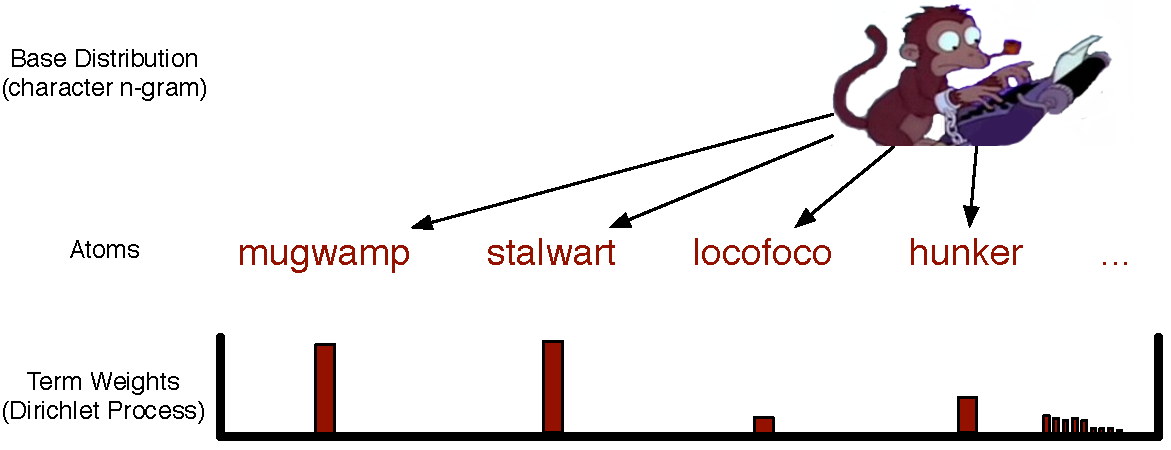
\includegraphics[width=.9\linewidth]{onlineag/dp_monkey-11}
    }
    \only<2->{
      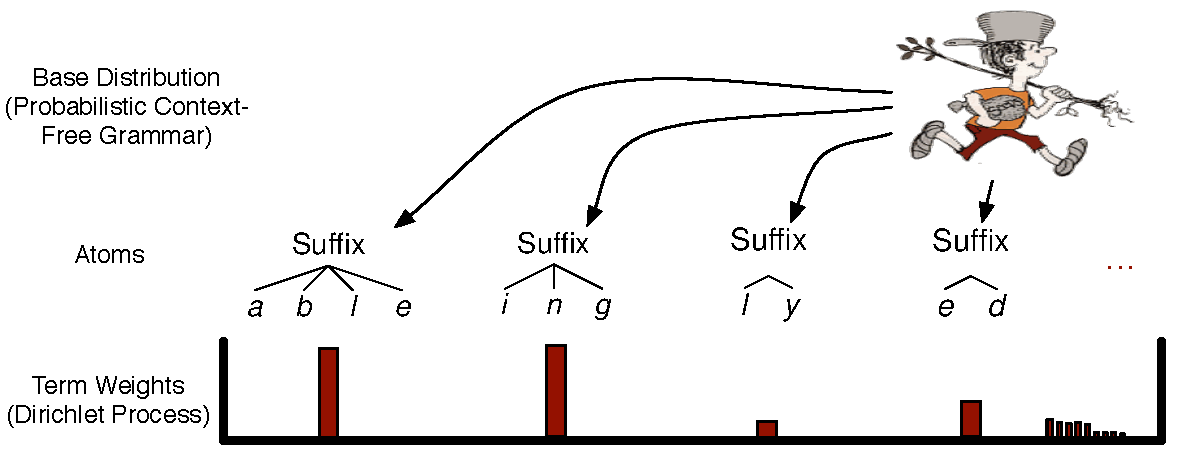
\includegraphics[width=.9\linewidth]{onlineag/dp_johnny}
    }
    \vspace{-6mm}
  \end{center}

  \begin{block}{\only<1>{Topic Models with Infinite Vocabulary}\only<2->{Adaptor Grammars: Nonparametric \textsc{PCFG}}}
    % \vspace{-5mm}
    \begin{center}
      % \resizebox{\linewidth}{!}{
      \begin{tabular}{r c}
        \only<1>{words}\only<2->{\sout{words} \alert{trees}}: &
        $\textstyle \rho_i \sim G_0$ \\
        weights: & $\textstyle b_i \sim \mathsf{Beta}(1,
        \alpha^\beta), ~ \textstyle \beta_i \equiv b_i
        \prod_{j=1}^{i-1} (1-b_j)$ \\
        \only<1>{topic}\only<2->{\sout{topic} \alert{grammaton}}: &
        $\textstyle G \equiv \sum_i \beta_i \delta_{\rho_i}$
      \end{tabular}
    \end{center}
    % }
    \vspace{-4mm}
    \only<1>{
      \begin{itemize}
      \item Base distribution $G_0$: $n$-gram model on characters.
      \item Topic: a distribution over words.
      \end{itemize}
    }
    \only<2->{
      \begin{itemize}
      \item Base distribution $G_0$: underlying \textsc{PCFG}.
      \item Grammaton: a distribution over derivation trees.
      \end{itemize}
    }
  \end{block}
\end{frame}

\begin{frame}{Word Segmentation $F_1$ Score}
  \vspace{-5mm}
  \begin{columns}

    \column{0.35\linewidth}
    \begin{center}
      % \resizebox{\linewidth}{!}{
      % \begin{tabular}{c | c | l}
      %   \hline
      %   \multirow{9}{*}{\begin{turn}{90}\emph{collocation}\end{turn}} &
      %   & \AgRule{ \AgNonTerm{Sent}{} }{ \AgNonTerm{Colloc}{} } \\
      %   & & \AgRule{ \AgNonTerm{Sent}{} }{ \AgNonTerm{Colloc}{} \AgNonTerm{Sent}{} } \\
      %   & & \AgRule{ \AgAdNonTerm{Colloc}{} }{ \AgNonTerm{Words}{} } \\
      %   \cline{2-3}
      %   & \multirow{6}{*}{\begin{turn}{90}\emph{unigram}\end{turn}}
      %   & \AgRule{ \AgNonTerm{Words}{} }{ \AgNonTerm{Word}{} }{} \\
      %   & & \AgRule{ \AgNonTerm{Words}{} }{ \AgNonTerm{Word}{} \AgNonTerm{Words}{} }{} \\
      %   & & \AgRule{ \AgAdNonTerm{Word}{} }{ \AgNonTerm{Chars}{} }{} \\
      %   & & \AgRule{ \AgNonTerm{Chars}{} }{ \AgNonTerm{Char} }{} \\
      %   & & \AgRule{ \AgNonTerm{Chars}{} }{ \AgNonTerm{Char}{} \AgNonTerm{Chars}{} }{} \\
      %   & & \AgRule{ \AgNonTerm{Char}{} }{ \AgNonTerm{$\star$}{} }{} \\
      %   \hline
      % \end{tabular}
      % }

      \resizebox{\linewidth}{!}{
        \begin{tabular}{l}
          \hline
          \AgRule{ \AgNonTerm{Words}{} }{ \AgNonTerm{Word}{} }{} \\
          \AgRule{ \AgNonTerm{Words}{} }{ \AgNonTerm{Word}{} \AgNonTerm{Words}{} }{} \\
          \AgRule{ \AgAdNonTerm{Word}{} }{ \AgNonTerm{Chars}{} }{} \\
          \AgRule{ \AgNonTerm{Chars}{} }{ \AgNonTerm{Char} }{} \\
          \AgRule{ \AgNonTerm{Chars}{} }{ \AgNonTerm{Char}{} \AgNonTerm{Chars}{} }{} \\
          \AgRule{ \AgNonTerm{Char}{} }{ \AgNonTerm{$\star$}{} }{} \\
          \hline
        \end{tabular}
      }

      \vspace{2mm}
      $h$ $o$ $w$ $a$ $r$ $e$ $y$ $o$ $u$

      \vspace{2mm}
      \resizebox{\linewidth}{!}{
        \Tree [.Words \qroof{ $h$ $o$ $w$ }.Word [.Words \qroof{ $a$ $r$
          $e$ }.Word [.Words \qroof{ $y$ $o$ $u$ }.Word ] ] ]
      }
    \end{center}

    \column{0.625\linewidth}
    \begin{center}
      \onslide<2->{
        \emph{brent} corpus\\
        % \begin{figure}[!tb]
        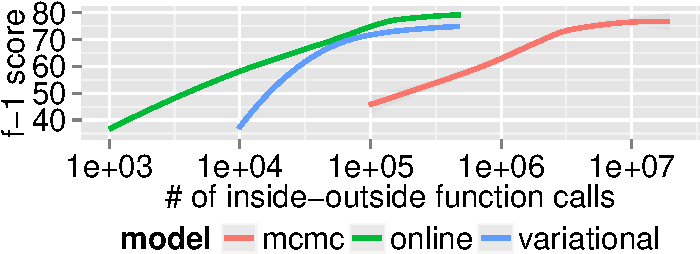
\includegraphics[width=1.0\linewidth]{onlineag/brent-Gunigram-log-crop.pdf}
        % \end{figure}
        % unigram grammar
        % \begin{figure}[!tb]
        %   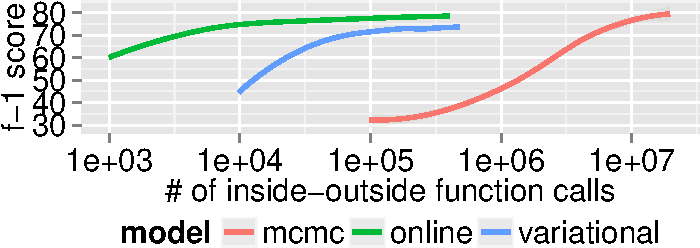
\includegraphics[width=1.0\linewidth]{onlineag/brent-Gcollocation-log-crop.pdf}
        % \end{figure}
        % collocation grammar
      }

      \onslide<3->{
        \vspace{2mm}
        Chinese Word Segmentation\\
        \resizebox{\linewidth}{!}{
          \begin{tabular}{ c | c | c c c }
            \multicolumn{2}{c|}{} & \emph{ctb7} & \emph{pku} & \emph{cityu} \\
            \hline
            \multirow{3}{*}{\begin{turn}{90}\shortstack{Data\\Facts}\end{turn}}
            & \# sentenses & $162k$ & $183k$ & $207k$ \\
            & \# word types & $57k$ & $53k$ & $64k$ \\
            & \# char types & $4.5k$ & $4.6k$ & $5k$ \\
            \hline
            \multirow{3}{*}{\begin{turn}{90}\shortstack{F$_1$\\Score}\end{turn}}
            & \abr{mcmc} & $71.75$ & $71.04$ & $74.01$ \\
            & \abr{online} & $72.82$ & $72.14$ & $74.71$ \\
            & \abr{variational} & $69.83$ & $67.82$ & $70.47$ \\
            \hline
          \end{tabular}
        }
      }
    \end{center}
  \end{columns}
\end{frame}

\begin{frame}{Summary}
  \begin{itemize}
  \item Propose adaptor grammars with online hybrid inference\\
    \begin{scriptsize}
      \bibentry{zhai-14c}
    \end{scriptsize}
    % \begin{itemize}
    % \item faster inference, scalable to larger datasets
    % \item flexible hierarchy, prototyping Bayesian model
    % \end{itemize}
  \item Demonstrate how efficient and effective our proposed inference
    method is comparing to all past approaches.
  % \item Also available in~\citet[TACL]{zhai-14c}\ldots
  %   \begin{itemize}
  %   \item Detailed explanations on online hybrid inference
  %   \item Heuristics on ordering and pruning of grammatons
  %   \item Experiments using hierarchical grammars
  %   \item Explore sensitivity to parameter settings
  %   \item Prototype \textsc{InfVoc} topic model using adaptor grammars
  %   \item Qualitative and quantitative results on the prototyped model
  %   \end{itemize}
  \item Source code available at my github repo.
  \end{itemize}
\end{frame}
